As it is mentioned DSL (Chapter \ref{ch:fundamentals}), After research and looking for suitable existing state modeling languages, it has been decided to create a new DSL based on run-time state migration requirements.
A DSL can be developed from scratch, or it can be a modification or a modified form of an existing domain-specific modeling language.

The Application State Modeling Language (ASML) is a DSL that defines any software application state.
The focus of this language is on modeling states of the run-time.

An application can have multiple states and users can switch between them.
These states and their transition can be a modeled in different ways (e.g, UML state machine diagram), but as we deal with the data perspective and have to access to the actual values and migrate them, we need a structured language for defining states (e.g, Amazon States Language). As the actual data of a state will be migrated, there is no need to include transition between states and each model is able to covers only an individual state. As mentioned in requirements (Chapter \ref{ch:requirements}), this language supports states that are migratable.
It is not supporting the transition between states as we assume we know in which state application is. 

The advantage of having an individual model for each state is improving interoperability, allowing different domain applications to share a specific part of them.
For example, an email domain application has a calendar that can migrate data with a phone calendar application.
Also, there is no need to model the states which are not migratable. So, it reduces the time of modeling state and the amount models. 

The model in ASML is called Application State Model, which is discussed in subchapter 5.2.

The actual value of the state is Run-Time State which is discussed in subchapter 5.3.
\subsection{Metamodel}

Figure \ref{fig:asml-meta-model} shows the metamodel of our DSL as an UML class diagram. A mapping document can describe one state. Each state  specified in the mapping document has a unique name. The extra information of a state are version and author that they can be defined in Number and String. Each state can have multiple attributes. Each attribute consist of a unique name and a specific content which its type can be a primitive types like Array, Object, Boolean, File, Number and String. 

\todo{change attribute to value}

\begin{figure}
    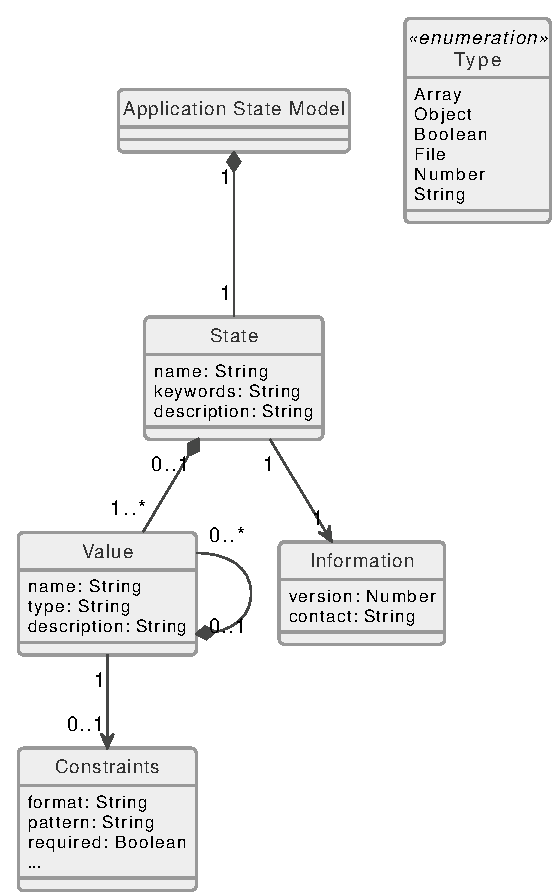
\includegraphics[scale=1]{../figures/asml-class-diagram}
    \centering
    \caption{UML Class Diagram of our DSL Metamodel}
    \label{fig:asml-meta-model}
\end{figure}

\subsection{Language Stack}
There are so many ways to define a DSL; it can be made from scratch (e.g., developing a language base on Xtext framework) or extended or restricted versions of other languages. The ASML is introducing a syntax based on JSON and is a extended version of JSON Schema. 


\subsubsection{JSON Schema}
After the tremendous popularity of JSON, some scenarios could benefit from a declarative way of defining a schema for JSON documents.
A declarative schema specification would give programming languages and developers a standardized language to specify what types of JSON documents are valid as inputs and outputs \cite{json-schema}.

The schema can be another JSON document that defines acceptable key-value pairs.
For instance, the simple JSON document in Listing \ref{lis:json}, can be declare in JSON Schema document in Listing \ref{lis:json-schema}

\lstset{
  label=lis:json-schema, caption=A simple JSON Schema document.
}
\begin{lstlisting}[language=json]
{
    "properties": {
        "fullname": {
            "type": "string"
        },
        "email": {
            "type": "string",
            "format": "email"
        }
    }
}
\end{lstlisting}

JSON Schema can define a document must have several properties, including regular data-types like objects, arrays, strings, booleans, numbers and, null. Each of these types has different keywords that help to specify and restrict the schema. The most important attribute is “type” whose value is defining the schema. Constraints can be applied on an instance by adding validation keywords to the schema \cite{json-model}. For example in Listing \ref{lis:json-schema}, \lstinline[basicstyle=\ttfamily]|{"type": "string"}| specify a value with string type.

In this thesis, for readability reasons we use YAML syntax to represent the Application State Model in JSON Schema. YAML is a human-readable syntax and can be converted to JSON syntax without extra configuration. Listing \ref{lis:yaml-simple} shows a simple example based on Listing \ref{lis:json-schema} which is a JSON Schema document.

\lstset{
  label=lis:yaml-simple, caption=Example of expressing JSON Schema in YAML syntax., 
}
\begin{lstlisting}[language=yaml]
properties:
  fullname:
    type: string
  email:
    type: string
    format: email
\end{lstlisting}

\subsection{Language Schema}
The Application State Language itself is a JSON Schema document based on JSON Schema Draft-07
\footnote{\href{https://json-schema.org/draft-07/json-schema-release-notes.html}{JSON Schema Draft-07 Release Notes}}
and is following the same logic and syntax. Table \ref{tab:asml-schema} shows the schema of ASML. 
The full schema of ASML is available on its GitHub repository
\footnote{\href{https://github.com/asml-lang/asml/blob/master/schemas/schema.json}{https://github.com/asml-lang/}}.

\subsubsection{Mapping Metamodel to JSON Schema}
The metamodel of ASML (Fig. \ref{fig:asml-meta-model}) is mapped in JSON Schema. The mapping document can be considered as a JSON Schema document which is a model. Therefore, each state should be defined in one JSON Schema document. Attributes of a state are mapped to \lstinline[basicstyle=\ttfamily]{properties} element of JSON Schema, which each attribute should have a unique name as key and its data type can be defined as a key-value pair. The content of a attribute is mapped to a actual value in a JSON document, which they are objects. The extra information like version and author's contact are mapped to \lstinline[basicstyle=\ttfamily]{info} element.


\begin{table}
\begin{tabularx}{\textwidth}{|l|X|X|r|}
\hline
Property             & Description                                                                              & Value                                                                                                                   \\\hline
title                & The name of the DSL.                                                                     & Application State Modeling Language                                                                                     \\\hline
description          & The description of the DSL.                                                              & A DSL for enabling run-time state migration between same-purpose applications of different vendors \\\hline
version              & The current version of the DSL, which can be used in for version checking for validating models. & 1.0.0                                                                                                                   \\\hline
properties           & Contains properties which a model should have.                                       & \{"asml", "info", "properties", "required"\}                                                                            \\\hline
required             & Defining the requited items which a model must have.                                     & {[}"asml", "info", "properties"{]}                                                                                      \\\hline
additionalProperties & The DSL is not allowing developers to add additional properties to models.               & false                                                                                                                   \\\hline
definitions          & Contains the definition of the DSL items and the basic JSON Schema specification.        & version, asml, info, contact, Schema

\\\hline
\end{tabularx}
\caption{ASML Schema}
\label{tab:asml-schema}
\end{table}





